\documentclass[a4paper, 11pt, titlepage]{article}
% \usepackage{geometry}
% \usepackage{longtable}
\usepackage{tabularx}
\usepackage{setspace}
\usepackage[backend=biber]{biblatex}
\usepackage{bm}
\usepackage{amsmath}
\usepackage{hyperref}
\usepackage{graphicx,float}
\addbibresource{references.bib}

% \nocite{*}

\newcommand{\vmiddle}[1]{\begin{tabular}{l} #1 \end{tabular}}
\renewcommand\tabularxcolumn[1]{m{#1}}% for vertical centering text in X column
\renewcommand\i[1]{\textit{#1}}% for vertical centering text in X column

\title{COMP4906\\
Honours Thesis Proposal\\
A Real-Time Fluid Simulation Framework for Fluid-Geometry Interaction in Game Environments}
\author{Gabriel Racz}
\begin{document}
\maketitle

\section{Objective}
In recent years, modern graphics hardware has improved at a rate far exceeding
the relative improvements in CPU capabilities. This, along with the development
of more powerful graphics APIs exposing general purpose computation, has lead to
modern game engines utilizing the GPU to vastly increase visual fidelity and
immersion in real-time games. The addition of indirect draw calls generated from within
compute shaders has allowed GPU driven rendering to render scenes with an
order of magnitude higher scene complexity and object counts compared to
traditional CPU approaches, dedicated hardware ray tracing cores have enabled
photorealistic lighting and global illumination by modeling physically-based
light transport, and flexible compute shaders have been used to simulate
physical phenomena and procedural animation of game assets such as hair, cloth,
and vegetation.

One area of computer graphics that has not seen as wide adoption in
real-time games is physically-based volumetric effects. This is in part due to
the high memory and compute requirements associated with storign, simulating
and rendering volumetric grids. Techniques for modelling gaseous fluids
such as smoke and fire have remained relatively constant over the years, relying
on simple particle systems, sprite billboarding, and pre-rendered animations to give the illusion of
volumetric effects. Although relatively cheap and effective for small
assets, this approach often breaks down when modelling medium to large flows
that encompass a scene or interact with the scene geometry. Similarly, wind
systems are often implemented with scrolling noise textures that are effective
for approximating global interactions in wide open scenes, but do not capture
flow around large game objects such as trees and buildings.

Specific games examples.
God of war did a simple diffusion-based wind simulation for cloth, hair
vegetation.
Ghost of Tsushima did noise wind effects, 2D
Both not geometry interaction
Billboarding for flames, smoke, god rays (illumination),
CS2 volumetric smoke

For many games, these fluids are of secondary concern to the main gameplay and
visuals, justifying their simple and cheap approaches. However, there are also
many opportunities for creating unique player experiences by taking full
advantage of dynamic general volumetric scene representation. Blah blah blah
give some examples of cool stuff we can do. Billowing smoke and fog, 





% The objective of my thesis will be to develop a framework for efficient
% GPU gaseous fluid simulation for the use in real-time games with a focus on geometry-fluid
% interaction. This will include the development of a dynamic player-centered
% sparse grid which will be incrementally refined around game geometry and areas of
% high fluid detail. Other requirements are as follows:
% \begin{itemize}
%     \item Create visually interesting physically-based fluid flow around complex
%     geometry
%     \item End-to-end computational and memory efficiency suitable for
%     integration into production game engines
%     \item Volumetric rendering of fluid data incorporating light scattering
%     \item GPU voxelization/simplification of scene geometry into the fluid domain
%     \item Leverage modern GPU compute capabilities using Vulkan to implement
%     methods found during literature review
% \end{itemize}


\section{Fluid Dynamics Background}
\subsection{Equations of Motion}

A fluid with constant density and temperature can be modelled by a velocity
vector field $\bm{u}$ and a scalar pressure field $p$. These fields respectively
represent the  instantaneous velocity vector
and outwards pressure force at any point within the fluid domain. A set of
famous partial differential equations called the \i{incompressible
Navier-Stokes} equations describe the evolution of an incompressible fluid over time.

\begin{equation}\label{nsmomentum}
    \frac{\partial \bm{u}}{\partial t} + (\bm{u} \cdot \nabla)\bm{u} = - \frac{1}{\rho}\nabla p + \nu \nabla^2\bm{u} + \bm{f} \\
\end{equation}
\begin{equation}\label{nsincomp}
    \nabla \cdot \bm{u} = 0
\end{equation}

Equation \eqref{nsmomentum} is analogous to Newton's momentum
equation $F = ma$ from classical mechanics. It describes the relationship between force and motion for a
continuous fluid medium rather than discrete point particles. Equation
\eqref{nsincomp} is the incompressibility constraint on the velocity field. It states that the \i{divergence} of the velocity field should
be 0 at every point in space, ensuring that the fluid conserves mass over time.

Each term from the momentum equation governs a different aspect of fluid
behavior which when combined produces complex flow patterns. Seeing as these
are the basis for all preceding research, it is worth describing
their individual contributions.

The simplest of the terms $\bm{f}$ is the \i{external force}. This force
incorporates outside influences acting on the system. Oftentimes this includes
gravity, as well as artist-driven inputs.

The \i{viscous} term $\nu \nabla^2\bm{u}$ accounts for the internal friction
within the fluid. It acts to diffuse the fluid velocity overtime, causing
neighbouring regions to ``drag'' against each other, gradually bringing the
system to a more uniform state. The Laplacian operator $\nabla^2$ when applied
to $\bm{u}$ yields a new vector field representing the spatial variation of the
velocity. Multiplying by the fluid's viscosity constant $\nu$ updates
local regions to be more inline with their neighbours.

$-\frac{1}{\rho}\nabla p$ is the pressure gradient term. It
describes the change in fluid velocity due to the differences in pressure inside
of the fluid. The pressure gradient $\nabla p$, force per unit volume, is
divided by the fluid density $\rho$ to obtain the acceleration due to this
difference in pressure (similar to $a = \frac{F}{m}$). The term is negated as
the fluid naturally moves from areas of high to low pressure. As we will show
later, this term is crucial in satisfying the incompressibility constraint
\eqref{nsincomp}

Finally the convective term $(\bm{u} \cdot \nabla)\bm{u}$ represents the
transport of momentum due to the fluid's own motion. Commonly called
\i{advection}, this models the movement of the fluid along the velocity field. The differential operator $(\bm{u} \cdot
\nabla)$ encodes how the velocity changes as you follow a fluid particle's path,
which we then apply to the velocity field itself.
Notably this results in a nonlinear as the evolution of the velocity field overtime
depends on its own spatial derivatives.

\subsection{Incompressibility}
In computer graphics applications, fluid simulations are generally performed under the
assumption of incompressibility, where the density of the fluid remains constant
throughout the flow. This vastly simplifies the
Navier-Stokes equations for general compressible fluids which are otherwise
complex and expensive to compute, yielding the simplified form described
above. Under non-extreme circumstances, the
effects of compressibility are negligible for the simulation of visually
appealing flow behaviors. To ensure that the fluid satisfies the
incompressibility constraint \eqref{nsincomp} however, we must ensure that
updates made to the system via the momentum equation \eqref{nsmomentum} also
maintains the divergence-free property. This step is commonly referred to as the
projection step. The intermediate velocity field $\bm{u}^*$ obtained from
solving the previously discussed advection, viscous, and external terms is \i{projected} onto a
divergence-free representation of itself.

Various methods have been proposed for the solution of this projection step with
various tradeoffs in physical accuracy and computational efficiency. One early method
leveraged by Jos Stam \cite{stam2003real} relies on the Helmholtz-Hodge Decomposition theorem,
stating that any vector field $\bm{w}$ can be uniquely decomposed
into the form
\begin{equation}
    \bm{w} = \bm{u} + \nabla q
\end{equation}
where $\bm{u}$ has zero divergence and $q$ is a scalar field, effectively
splitting the field $\bm{w}$ into its \i{curl-free} and \i{gradient-free} components. The
equation can be rewritten in two terms by multiplying both sides by $\nabla$, removing
the $\bm{u}$ term since $\nabla \cdot \bm{u} = 0$.
\begin{equation}\label{poisson}
    \nabla \cdot \bm{w} = \nabla^2 q
\end{equation}
This equation is a Poisson Equation for the field $q$, the solution of which
allows us to ``correct'' our intermediate velocity field $\bm{u}^*$ by removing
its divergence component. Stam used this strategy to define a projection
operator $\bm{P}$ that computes the projection $\bm{u}$:
$$
    \bm{u} = \bm{P}\bm{w} = \bm{w} - \nabla q
$$
Applying the operator $\bm{P}$ to the momentum equation \eqref{nsmomentum}, and
using the fact that $\bm{P}\bm{u} = \bm{u}$ due to the incompressibility constraint
and $\bm{P}\nabla p = 0$ as it is a pure gradient field,
obtains a single equation governing the change in the fluid velocity over
time
\begin{equation}
\begin{aligned}
    \frac{\partial \bm{u}}{\partial t} &= \bm{P}\left(-(\bm{u} \cdot \nabla)\bm{u} + \nu\nabla^2\bm{u} + \bm{f}\right) \\
    \frac{\partial \bm{u}}{\partial t} &= \bm{P}\left(\bm{u}^*\right) - \nabla q \\
\end{aligned}
\end{equation}

Later, authors such as Fedkiw \cite{fedkiw2001visual} and Bridson \cite{bridsonbook} applied a
similar method to obtain projection operators that repurposed the pressure term
from the momentum equation to analogously replace $q$ in Stam's derivation. Namely, Fedkiw
incorporated the change in time $\Delta t$ with:
$$
    \bm{u} = \bm{u}^* - \Delta t \nabla p
$$

and Bridson incorporated the fluid density
$$
    \bm{u} = \bm{u}^* - \frac{\Delta t}{\rho} \nabla p
$$

Solving the Poisson equation of the form
\eqref{poisson} to obtain the corrective pressure gradient is largely the most
expensive step for a typical fluid solve \cite{bridsonbook}, requiring efficient
parallelization and discretization of the fluid domain.

\subsection{Lagrangian and Eulerian Viewpoints}
With the continuum of the fluid defined above, tracking its motion and evolution
over time requires a discretization of the domain. For fluids, there are two
categories that  each lead to different methods for solving
the Navier-Stokes equations: the Lagrangian frame and the Eulerian frame.

The Lagrangian viewpoint treats the fluid volume as a particle system where each
point in the fluid is represented as a seperate particle with position $\vec{x}$ and
velocity $\vec{v}$. The fluid behaviour is then governed by the interaction of
these discrete particles. In computer graphics, the particle system updates the
particles similar to classical mechanics, where the collisions and other local
forces between molecules are integrated over time to update the system.

The Eulerian viewpoint instead looks at fixed points in space and measures how the
fluid quantities such as density, and velocity change over time. This can be
thought of as discretizing the fluid domain into a static grid, where each grid cell
contains measurements on what the underlying fluid is doing at a given time.

Both of these methods give rise to different strategies when solving the fluid
equations and are each suited to different applications. The Lagrangian approach
naturally lends itself to the simulation of liquid, as the particle-based
representation makes it straightforward to capture the free surface of the
fluid, individual droplets, and splashes. This is mainly due to the minimal
computational overhead required to track the fluid interface when compared with
a grid based approach, as well as liquid particles behaving more closely to a
solid at the microscopic level. Methods such as SPH \cite{koschier2020smoothed}
and vortex methods \cite{park2005vortex} smooth
these discrete particles together to form a continous medium, while the updates
are performed at a per-particle basis. The Eulerian viewpoint are often more
commonly used in computer graphics due to the easier computation of local
quantities such as the pressure gradient and diffusion. It is significantly
easier to take spatial derivates on a fixed grid than in a cloud of arbitrarily
moving particles. Many methods leverage the strengths of both by using a hybrid
approach such as PIC/FLIP\cite{salomonsson2011pic} where particles carry fluid quantities but are
transferred to an underlying grid for the computation of spatial derivations. In
modelling incompressible flow, a semi-Lagrangian approach is taken to perform
stable advection of the fluid, simplifying the computation of the advection term.

\section{Literature}
\subsection{Stable Incompressible Fluids}
Stam's Stable Fluids paper \cite{stam2023stable} builds upon the work of Foster and Metaxas
\cite{foster1997modeling} to provide the first stable numerical solution to the incompressible
Navier-Stokes equations for the purposes of real-time applications. His insight
was to use the \i{method of characteristics} to solve the self-advection of the
fluid by adopting a semi-Lagrangian frame. Rather than solving the nonlinear
advection term using finite differencing as was done by Foster and Metaxas, he
traced the path of representative particles, centered on each grid cell, to
compute the motion of the fluid due to its own flow. Tracing grid particles
forwards in time however leads to numerical instability due to accumulating
interpolated velocities at the particles' cell destinations. Instead, he proposed
to trace the particle's motion backwards in time along the velocity field to
find the representative particle that would end up at each grid cell's center.
This has the benefit of ensuring each grid cell is updated by exactly one
particle which is perfectly aligned to the fluid grid, and moving the
interpolation to the representative particle starting location step. The
advection term is updated by:
$$
    \bm{u}_{\text{new}} = \bm{u}\left(\bm{p}(\bm{x}, -\Delta t)\right)
$$
where $\bm$ returns the position of the the particle at $\bm{x}$ advected
backwards in time through the velocity field $\bm{u}$. He claims that this
improvement makes the self-advection unconditionally stable for all
velocities and time steps, and extremely desirable property for real-time
fluids. Almost all preceding research on fluids for computer graphics leverages
this powerful property.

Stam also introduces a method for visualizing the otherwise constant density
fluid by incorporating a second dye, or smoke fluid quantity into the system.
This smoke is allowed to have variable density at different points in space,
advecting along the velocity field $\bm{u}$ with the same advection principal
described above, as well as diffusing throughout the medium using the same
viscous term found in \eqref{nsmomentum}

In Visual Simulation of Smoke \cite{fedkiw2001visual}, Fedkiw et. al proposed various
improvements on Stam's method. Due to the nature of using a discretized grid to
model a continuum such as a fluid, small-scale turbulent structures and high
frequency details are lost due to numerical dissipation. Once details fall below
a resolution that can ``escape'' a single grid cell, they are lost to the
diffusive properties of the grid updates. To reintroduce these details to the
fluid, Fedkiw et al. applied a method invented by Steinhoff \cite{steinhoff1994modification} for CFD called
\i{Vorticity Confinement}. In incompressible flow, the vorticity of the velocity
field is defined by:
$$
    \bm{\omega} = \nabla \times \bm{u}
$$
This is also called the curl of the velocity field $\bm{u}$. This vector field
describes the local spinning motion of each region within $\bm{u}$, similar to a
paddle wheel spinning the flow in a certain direction. We can leverage the curl
to adding forces back into the system after that have been lost due to the
damping in our coarse grid solutions, recovering some of the
small-scale turbulent behavior. By taking the normalized gradient of the curl
\begin{equation}
\begin{aligned}
    \bm{\eta} &= \nabla \vert\omega\vert \\
    \bm{N} &= \frac{\bm{\eta}}{\vert \bm{\eta} \vert}
\end{aligned}
\end{equation}
We obtain the vectors that point from areas of low vorticity to areas of higher
vorticity. By projecting back into the velocity field, we can add an amount of
vorticity that would be transported by the field
\begin{equation}
    \bm{f}_\text{vorticity confinement} = \epsilon h (\bm{N} \times \omega)
\end{equation}
where $\epsilon \> 0$ is a user-controlled parameter indicating the desired strength of
the confinement, and $h$ is the grid cell spacing.

Fedkiw et.al also improve upon the stable advection interpolation as described
by Stam by using a higher order cubic \i{Hermite} interpolation scheme rather
than the simple linear interpolation implemented by Stam. By considering more
control points when interpolating the particle's initial position the numerical
diffusion, (blurring) is reduced between solver time steps, further contributing
to the preservation of small-scale turbulence. Other interpolation schemes such
as B-Spline \cite{he2011real} can be substituted here, further increasing accuracy while
sacrificing computational efficiency.

He et. al built upon this work by introducing a method for spatially adaptive
vorticity confinement, where the vorticity is used to up-sample a coarse
velocity grid to improve performance. They also augment the vorticity
confinement to be proportional to the \i{helicity} of the fluid volume $V$ defined as:
$$
    H = \int \bm{u} \cdot \bm{\omega} dV
$$
which is a scalar field that represents the twisting of the flow around the
velocity vectors. This serves to add a spatially varying confinement coefficient
to the previously defined vorticity confinement equation when discretized
\begin{equation}
    \bm{f}_\text{vorticity confinement} = \epsilon h \vert \bm{u} \cdot \bm{\omega} \vert\left(\bm{N} \times \frac{\bm{\omega}}{\vert \bm{\omega} \vert}\right)
\end{equation}
They use this more accurate vorticity confinement method to allow discretizing
the velocity field over a relatively coarser grid by up sampling it and
retrieving the lost turbulent forces due to the increased damping caused by the
lower resolution.

As shown previously show, solving for the pressure force required to maintain
incompressibility between velocity field updates requires solving the poisson
equation
$$
\nabla^2p = \nabla \cdot \bm{u}^*
$$

When discretized to a grid, this equation is equivalent to a linear system
$$
    Ap = b
$$
where $A$ is the Laplacian operator $\nabla^2$, $p$ is the unknown pressure
field we are solving for, and $b$ is the velocity divergence field $\nabla \cdot
\bm{u}$. Bridson shows the derivation for the solution to this linear system
being equivalent to a finite differencing in each spatial
direction \cite{bridsonbook}.

The divergence of the velocity field represents the net flow entering/exiting
each cell of $\bm{u}$. Stam implemented simple central finite differencing in
his 2D fluid simulation as using the following formula:
\begin{align*}
    \nabla \cdot \bm{u}(x, y) &= \frac{\bm{u}(x + h, y) - \bm{u}(x - h, y)}{2h} + \frac{\bm{u}(x, y + h) - \bm{u}(x, y - h)}{2h}\\
\end{align*}
where $h$ is the grid cell separation. While efficient and simple to implement,
Bridson notes that this formulation has a a glaring numerical weakness \cite{bridsonbook} -- the
value of $\bm{u}(x, y)$ is never considered when computing its own divergence.
This makes it possible for the cell $\bm{u}(x, y)$ to be quite different from
its neighbours while still seemingly reporting a derivative of 0. Seeing as
though it is quite possible for the fluid domain to exhibit sharp variations
such as these, we need a method that will report the divergence more accurately
to enforce incompressibility. Ideally, we would like to be able to compute
\begin{align*}
    \nabla \cdot \bm{u}(x, y) &= \frac{\bm{u}(x + h/2, y) - \bm{u}(x - h/2, y)}{h} + \frac{\bm{u}(x, y + h/2) - \bm{u}(x, y - h/2)}{h}\\
\end{align*}
however this would lead to sampling the velocity grid along its separating
faces, and not in the cell centers where the velocity is stored.
To obtain an accurate and unbiased second-order central difference, Bridson employs
the use of a MAC grid \cite{harlow1965numerical}.

This grid structure staggers the velocity grid relative to the pressure grid, storing
the velocity vector components on the corresponding faces of their pressure grid cell.

\begin{figure}[H]
  \centering
  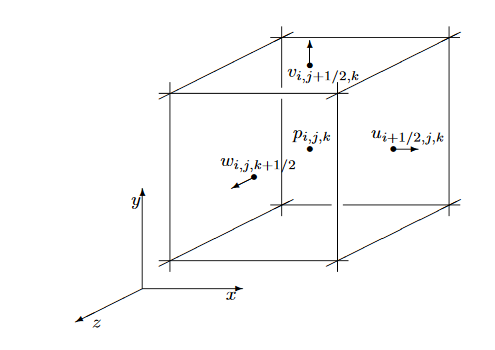
\includegraphics[width=0.5\linewidth]{MAC grid.png}
  \caption{One cell from the three-dimension MAC grid as published in \cite{bridsonbook}}
\end{figure}

The MAC grid structure greatly improves the stability of the pressure calculation
and subsequent incompressibility constraints,
however it requires interpolation to evaluate the full velocity vector at any
point. Despite necessary interpolation, most modern incompressible fluid solvers, real-time or
otherwise use this representation.

The Laplacian matrix $A$ is a sparse symmetric which encodes the computation of the partial derivatives for
each of the pressure cells within $p$ using a similar finite differencing
scheme. Each row $i$ of the Laplacian computes the partial derivative of its
corresponding pressure cell. In 3D, the diagonal of the Laplacian stores
coefficient $-6$ (as each cell has 6 neighbours to difference), and each row
contains mostly 0s, except in the columns corresponding to that row's neighbours
where 1s are stored. Seeing as it is so sparse, it is prohibitively inefficient
to store the entire Laplacian in memory -- in three dimensions its size is cubic relative to
the size of the pressure matrix -- the solution of the Poisson equation is
performed iteratively.

The solution to systems containing five- or seven-point Laplacian problems have been
exhaustively studied, as they appear in countless problems throughout engineering
and science. Thus, there are many numerical methods available, each with tradeoffs to
performance and accuracy. Simple methods such as various forms of the Jacobi iteration method
\cite{gomes2009linear} Gauss-Seidel relaxation \cite{gomes2009linear},and
Successive Over-Relaxation \cite{hadjidimos2000successive}, have
often been used in computer graphics applications where accuracy is not a priority
applications due to their low complexity, however
they suffer in convergence time to an optimal solution. Other popular methods
for modern fluid simulation in VFX
include the Conjugate Gradient Method, Multigrid, and Domain
Expansion \cite{bridsonbook}. This is area requires further experimentation towards methods
that best satisfy the performance and accuracy requirements for real-time
fluids.

Once the pressure field $p$ is found, we subtract it from the intermediate
velocity field $\bm{u}^*$ to obtain the final incompressible fluid result for
the timestep.

\subsection{Boundary Conditions}
Handling interaction between solid geometry and fluids requires satisfying
additional constraints in the cells that contain solid structures. To prevent
fluid flow from entering a solid voxel cell we must ensure that the component of
the fluid velocity normal to the solid voxel boundary must be 0
$$
    \vec{u} \cdot \vec{n} = 0
$$
If the solid is moving through the fluid, we can update the
constraint to allow the fluid velocity to match the normal component of the
solid's velocity.
$$
    \vec{u} \cdot \vec{n} = \vec{u}_\text{solid} \cdot \vec{n}
$$
Since we are only limiting the fluid's velocity component relative to the
normal of the solid boundary, this is called the \i{no-stick} condition. It says
the tangential velocity of the fluid is unaffected by the solid boundary, and
assumes inviscid flow around it. Since the solid cell contains no fluid, and
the pressure field indicates how much force should be applied at each cell to
force the system to be incompressible, we also must populate solid boundary cells with
$p = 0$ to ensure that it does not exert a corrective force on neighbouring
fluid cells. Setting values of the boundaries directly is commonly known
as a \i{Dirichlet} boundary condition. Although straightforward, Dirichlet
boundary conditions have been shown to exhibit artifacts in the resulting fluid
solutions such as artificial pressure gradients at the boundaries. Modern
practice is to enforce \i{Neumann} boundary conditions on the pressure:
$$
\frac{\partial p}{\partial \vec{n}} = \nabla p \cdot \vec{n}
$$
which specifies the normal derivative of the pressure rather than the direct
value. To handle this, some have
suggested applying fluid quantities in areas that do not contain actual fluid
(such as solid boundaries) \cite{bridsonbook,fedkiw1999non}. These are usually referred to
as \i{ghost cells}, and allow us to use the solvers of the continuum equations
to implicitly handle other non-fluid behaviors. Bridson describes manually
setting the velocity and pressure values on solid boundaries in such a way that
the solution of the pressure gradient handles the Neumann boundary conditions
between the fluid and solid. His derivation reveals that setting the pressure at
the solid boundaries to:
$$
    p_\text{solid} = p_\text{fluid} - \frac{\rho \Delta x}{\Delta t}(u_\text{fluid} - u_\text{solid})
$$
creates a Neumann boundary condition that is handled by the same equations that
govern the fluid interior, assuming that $p_\text{fluid}$ is a neighbouring
fluid cell to $p_\text{solid}$ and $u$ is the separating MAC grid velocity face between them at the same
point in space. As previously mentioned, $\frac{\rho \Delta x}{\Delta t}$ is the scaling term applied to
the pressure Laplacian to account for density, timestep, and grid cell size.

This ``voxelized'' approach to handling solid-fluid interaction is efficient and
suits real-time applications that have considerable amounts of dynamic
geometry. With sufficiently tesselated meshes, labelling of the solid voxels
within the fluid structure can be performed at the cost of a single point
lookup on the geometry vertices. Otherwise, fast voxelization methods for
rasterizing input geometry directly into a dynamic grid structure can be applied
described in \cite{janssen2015fast} or \cite{fang2000hardware}.

% Level set methods
% Finite Volume methods
% Quadric error metric for mesh simplification
 
% Boundary conditions
\subsection{Sparse Dynamic Grids}
Uniform grids are often used for most basic 3D solvers due to their extremely
fast data access, contiguous memory layout, and ease of implementation. However,
they also carry several limitations that make them impractical for real-time
applications. One of these drawbacks is illustrated when simulating scenes where
the region of fluid occupies a relatively small area of the total simulation
domain. Large amounts of computation and memory are wasted on regions that have
little to no bearing on the updates to the active fluid region. This is less of
a problem for liquids, where a tight bounding box can be
translated between updates by predicting the motion of the liquid volume through
its previous velocity field. However, for simulation of gases, areas of
seemingly empty or inactive space still significantly contributes to the
solutions of pressure. To remedy this, various data structures to store
\i{sparse} representations of the fluid grid have been developed.

The simplest approach as described by Bridson is to use a sparse
blocked grid. In this implementation, he implemented a two-level grid hierarchy
where a coarse grid was used to tile to simulation domain, and subsequent ``fine
blocks'' -- storing tiny contiguous arrays -- could be assigned to areas of high
detail. He later extended his work by increasing the tree depth to 4 levels, and
adding a hashing index scheme to minimize the overhead introduced by the tree
index traversal \cite{bridson2003computational}.

Losasso et al. \cite{losasso2004simulating} implemented an octree data structure to adaptively
refine their simulation grid using various refinement criteria. They described
the following modifications to the Navier-Stokes equations in order to account
for the variation in volume between grid cells
\begin{equation}
    V_\text{cell} \nabla \cdot (\bm{u}^* - \Delta t\nabla p) = 0
\end{equation}
\begin{equation}
    V_\text{cell} \nabla \cdot (\Delta t\nabla p) = \sum_{\text{faces}}((\Delta t \nabla p)_\text{face} \cdot n)A_\text{face}
\end{equation}
Where $V_\text{cell}$ is the volume of a of their largest cell, is used to
construct a linear system to solve for pressure considering the area of each
adjacent face. They refined their octree structure prioritizing areas containing
solid geometry, vorticity at each grid cell, and a clamped density range just
above the visible limit while being low enough to warrant higher resolution.

Similarly, Lentine et. al \cite{lentine2010novel} applied a similar hierarchical tree
structure with two main differences. They subdivided a coarse grid
representation into finer uniform grids which allowed them to maintain efficient
linear truncated access at each grid level. They also opted to solve the
intermediary velocity updates on the finest grid resolution, and only utilized
the hierarchical representation to compute the pressure projection locally at
for each grid resolution. To supplement the detail lost, they also added
Kolmolgorov noise as done in \cite{rasmussen2003smoke} during upsampling of the
fine grid. Various other noise functions have been used to improve down sampling
detail from sparse grids and should be investigated \cite{kim2008wavelet,
bridson2007curl}.

Modern approaches to fluid simulation largely rely on the GPU to accelerate
highly parallel nature of the Eulerian Naviar-Stokes equations. A family of
methods focused on optimizing sparse dynamic grids in VRAM have been developed
in recent years based on the original paper VDB \cite{museth2013vdb}. DCGrid \cite{raateland2022dcgrid} is the
newest of these and implements a sparse adaptive grid that incorporates the
paging structure of modern GPU memory layouts. They put particular emphasis on
creating mip-mapped resolutions of the grid structure, as well as utilizing
apron cells around boundaries of changing resolutions to optimize stencil
operations which are common when solving the pressure and diffusion equations.

\subsection{Rendering}
Rendering volumetric data requires a different approach to traditional geometry.
The most common approach for rendering volumetric data is to use ray marching.
In the case of gaseous fluids such as smoke and fire, rays marched along the
fluid domain, accumulating radiance of each fluid cell they traverse.

Rasmussen et. al \cite{rasmussen2003smoke} introduce a few interesting
improvements over standard ray marching. They modified their simulation domain
to be cylindrical inline with the camera view frustum rather than rectangular,
resulting in each grid cell being a truncated pyramid. This has two ingenious benefits:
the ray marching algorithm which usually needs to perform a line-rasterizing
algorithm to traverse the grid cells is instead replaced by
simple cell index increments, and the refinement of the simulation domain near
the camera view is handled implicitly by the increasing cell sizes relative to
view distance. Finally, they mention that for high albedo medium such as smoke,
light scattering within the fluid volume becomes effectively isotropic and can be
modeled as a diffusion process. This along with other fluid quantities such as
temperature can be diffused by the efficient fluid solvers already in place.

\section{Schedule}
\begin{tabularx}{\textwidth}{|X|X|}
\hline
\textbf{Period} & \textbf{Milestones} \\
\hline
November 18 - December 1 & \multicolumn{1}{X|}{
    Implement adaptive surface voxelization of triangle meshes (COMP5115 final project)
}\\
\hline
December 2 - December 15 & \multicolumn{1}{X|}{
    Further literature review guided by proposal feedback
}\\
\hline
December 16 - December 29 & \multicolumn{1}{X|}{
    Finalize geometry pipeline rendering and basic volumetric renderer
}\\
\hline
December 30 - January 12 & \multicolumn{1}{X|}{
    Incorporate MAC grid finite differencing and Neumann boundary conditions
    from \cite{bridsonbook}
}\\
\hline
January 13 - January 26 & \multicolumn{1}{X|}{
    Augment fluid simulation to 3D
}\\
\hline
January 27 - February 9 & \multicolumn{1}{X|}{
    Update uniform grid structures and algortihms to support sparse dynamic grids
}\\
\hline
February 10 - February 23 & \multicolumn{1}{X|}{
    Begin implementation for adaptive dynamic grid and refinement around fluid
}\\
\hline
February 24 - March 9 & \multicolumn{1}{X|}{
    Finalize adaptive dynamic grid and improve volumetric renderer
}\\
\hline
March 10 - March 23 & \multicolumn{1}{X|}{
    Performance optimization, compile results for report
}\\
\hline
March 24 - April 6 & \multicolumn{1}{X|}{
    Write and submit final report draft
}\\
\hline
April 7 - April 20 & \multicolumn{1}{X|}{
    Update final report based on feedback, submit
}\\
\hline
\end{tabularx}
\pagebreak
\printbibliography
\end{document}